% \section{Experiments}\label{sec:ch5:experiments}
% In this section we examine the effectiveness of our invariant layer by testing
% its performance on the well known datasets (listed in the order of increasing
% difficulty):
% \begin{itemize}
  % \item MNIST: 10 classes, 6000 images per class, $28\x 28$ pixels per image.
  % \item CIFAR-10: 10 classes, 5000 images per class, $32\x 32$ pixels per image.
  % \item CIFAR-100: 100 classes, 500 images per class, $32\x 32$ pixels per image. 
  % \item Tiny ImageNet\cite{li_tiny_2017}: 200 classes, 500 images per class, 
    % $64 \x 64$ pixels per image. 
% \end{itemize}
% Our experiment code is available at \cite{cotter_learnable_2019-1}.

\section{Layer Introduction with MNIST}\label{sec:ch5:mnist}
\begin{table}[t]
  \renewcommand{\arraystretch}{1.4}
  \centering
  \mycaption{Architectures for MNIST hyperparameter experiments}{The activation
  size rows are offset from the layer description rows to convey the input and
  output shapes. The `project' layers in both architectures are unlearned, so all
  of the learning has to be done by the first two layers and the reshuffle
  layer.}
  \label{tab:ch5:mnist_arch}
  \subfloat[Reference Arch with $3\x 3$ convolutions]{%
    \label{tab:ch5:mnist_arch_conv}
    \begin{tabular}{c c}
      \toprule
      Activation Size & Layer Name + Info \\
      \midrule
      \begin{tabular}{@{}c@{}} % This supresses the space on the left and right
        $1\x 28 \x 28$ \\ $7\x 28\x 28$ \\ $7\x 14\x 14$ \\ $49\x 14\x 14$ \\ $49\x 7\x 7$ 
        \\ $2401\x 1$ \\ $10\x 1$ \\ $10\x 1$ 
      \end{tabular} &
      \begin{tabular}{@{}c@{}}
        conv1, $w \in \reals[7\x 1\x 3 \x 3]$ \\ maxpool1, $2\x 2$ \\ 
        conv2 $w \in \reals[49\x 7 \x 3\x 3]$ \\ maxpool2, $2\x 2$ \\ unravel \\
        project, $w \in \reals[2401\x 10]$ \\ reshuffle, $w\in \reals[10\x 10]$
      \end{tabular} \\
      \bottomrule
    \end{tabular}
  }\quad
  \subfloat[Invariant Architecture]{%
    \label{tab:ch5:mnist_arch_inv}
    \begin{tabular}{c c}
      \toprule
      Activation Size & Layer Name + Info \\
      \midrule
      \begin{tabular}{@{}c@{}} % This supresses the space on the left and right
        $1\x 28 \x 28$ \\ $7\x 14\x 14$ \\ $49\x 7\x 7$ \\ $2401\x 1$ \\ $10\x 1$
        \\ $10\x 1$ 
      \end{tabular} &
      \begin{tabular}{@{}c@{}}
        inv1, $A \in \reals[7\x 7]$ \\ inv2, $A \in \reals[49\x 49]$ \\ unravel \\
        project, $w \in \reals[2401\x 10]$ \\ reshuffle, $w\in \reals[10\x 10]$
      \end{tabular}\\
      \bottomrule
    \end{tabular}
  }
\end{table}




\begin{table}[hbt]
  \centering
  \mycaption{Hyperparameter settings for the MNIST experiments}{The weight gain is
  the term $a$ from \autoref{eq:ch5:glorot}. Note that $\log_{10} 3.16 = 0.5$.}
  \label{tab:ch5:hyper_options}
  \begin{tabular}{c c}
    \toprule
    Hyperparameter & Values \\
    \midrule
    Learning Rate (lr) & $\left\{ 0.0316,\ 0.1,\ 0.316,\ 1 \right\}$ \\
    Momentum (mom) & $\left\{ 0,\ 0.25,\ 0.5,\ 0.9 \right\}$ \\
    Weight Decay (wd) & $\left\{ 10^{-5},\ 3.16\x 10^{-5},\ 10^{-4},\ 3.16\x 10^{-4} \right\} $\\
    Weight Gain (a) & $\left\{0.5,\ 1.0,\ 1.5,\ 2.0 \right\}$
    \\\bottomrule
  \end{tabular}
\end{table}

\begin{table}[hbt]
  \centering
  \mycaption{Architecture performance comparison}{Numbers reported are the mean
  and standard deviation of accuracy over 10 runs with the optimal
  hyperparameters, $\theta$. Note that for
  both architectures we found that $\F{lr}$ was the most important
  hyperparameter to choose correctly, and had the largest impact on the
  performance.
  % We also use
  % fANOVA\cite{hutter_efficient_2014} analysis to weight the importance of these 
  % hyperparameters. High values imply the accuracy is more sensitive to this
  % hyperparameter. 
  }
  \label{tab:ch5:mnist_initial_results}
  \begin{tabular}{@{}l c c c@{}}
    \toprule
     & &\multicolumn{2}{c}{accuracy} \\\cline{3-4}
    Architecture & $\theta = \{\F{lr}, \F{mom}, \F{wd}, \F{a}\}$ & mean & std  \\\midrule
    Convolutional & $\{0.1,\ 0.5,\ 10^{-5},\ 1.5 \}$ & 97.3 & 0.29 \\
    Invariant & $\{0.032,\ 0.9,\ 3.2\x 10^{-5},\ 1.0 \}$ & 96.6 & 0.26 \\
    \bottomrule
  \end{tabular}
\end{table}

To begin experiments on the proposed locally invariant layer, we look at how
well a simple system works on MNIST and compare it to an equivalent system with
convolutions. Because of the small size of the MNIST challenge, we can quickly
get results, allowing a large number of trials and a broad search over
hyperparameters to be done. In this way, we can use the findings from these
experiments to guide our work on more difficult tasks like CIFAR and Tiny
ImageNet.

To minimize the effects of learning from other layers, we build a
custom small network, as described in \autoref{tab:ch5:mnist_arch}. 
The first two layers are learned convolutional/invariant layers, followed by
a fully connected layer with \emph{fixed} weights that we can use to project down to
the number of output classes. Finally, we add a small learned layer that
linearly combines the 10 outputs from the random projection, to give 10 new
outputs. This is to facilitate reordering of the outputs to the correct class.
This simple network is meant to test the limits of our layer, rather than
achieve state of the art performance on MNIST.

Given that our layer is quite different to a standard convolutional layer, we
must do a full hyperparameter search over optimizer parameters such as the
learning rate, momentum, and weight decay, as well as layer hyperparameters 
such as the variance of the random initialization for the mixing matrix $A$.

To simplify the weight variance search, we use Glorot Uniform Initialization
\cite{glorot_understanding_2010} and only vary the gain value $a$:
%
\begin{equation}
  A_{ij} \drawnfrom U\left[ -a\sqrt{\frac{6}{(C_l + C_{l+1})HW}},\ a\sqrt{\frac{6}{(C_l + C_{l+1})HW}}\
  \right] \label{eq:ch5:glorot}
\end{equation}
%
where $C_l,\ C_{l+1}$ are the number of input and output channels as before, and
the kernel size is $H = W = 1$ for an invariant layer and $H = W= 3$ for a
convolutional layer.

We do a grid search over these hyperparameters and use Hyperband
\cite{li_hyperband:_2016} to schedule early stopping of poorly performing runs.
Each run has a grace period of 5 epochs and can train for a maximum of 20
epochs. We do not do any learning rate decay.  We found the package Tune
\cite{liaw2018tune} was very helpful in organising parallel distributed training
runs.  
% Finally, we use fANOVA \cite{hutter_efficient_2014} analysis
% to find the importance of these hyperparameters to our layer, comparing to a
% standard layer. 
The hyperparameter options are described in
\autoref{tab:ch5:hyper_options}, note that we test $4^4=256$ different options.

Once we find the optimal hyperparameters for each network, we then run the two
architectures 10 times with different random seeds and report the mean and variance of
the accuracy. The results of these runs are listed in
\autoref{tab:ch5:mnist_initial_results}.


\subsection{Proposed Expansions}\label{sec:ch5:mnist_newlayer}
The results from the previous section seem to indicate that our proposed
invariant layer is a slightly worse substitute for a convolutional layer.

We posit that this is due to the centred nature of the wavelet bases that were
used to generate the $z$ and later the $y$ coefficients. As they are all centred
at roughly the same location (the phase of the complex wavelet allows for some
small spatial separation) $1\x 1$ convolutions may not be capable of building
richer shapes by separating the wavelet centres. This effect was seen in the
previous chapter when we presented some possible new shapes in
\autoref{fig:ch4:newshapes}. The bottom right quadrant were shapes made from
mixing wavelet coefficients in a $3\x 3$ area, and these were much richer than
those attainable by only mixing in a $1\x 1$ area\footnote{This comparison is
only a guide, however, as in this chapter we are mixing coefficients after taking
the modulus, whereas \autoref{fig:ch4:newshapes} were generated by mixing with
complex gains \emph{before} the modulus.}

To get spatial separation, we must replace the $1\x 1$ mixing kernel from
\eqref{eq:ch5:mixing} ($\tilde{\alpha}_f(q)$) with a $3\x 3$ filter $g_f(q,
\xy)$. We also change the multiply for convolution, giving us:
% \tilde{a}_f(q) \alpha_f(q, \xy) 
\begin{equation}
  y^{(l+1)}(f, \xy)  =  \sum_{q \in Q} z^{(l+1)}(q, \xy) \conv g_f(q, \xy)
\end{equation}

If all of the parameters of $g_f(q, \xy)$ are learned, then
the number of parameters in \eqref{eq:ch5:num_params} increases from $7C_l
C_{l+1}$ to $63C_l C_{l+1}$. This is quite a lot of parameters for a single
layer, and much more than the $9C_lC_{l+1}$ of a standard $3\x 3$ convolution, or
even the $25C_l C_{l+1}$ of a larger $5\x 5$ convolution.

However, we can still get spatial separation without having to learn \emph{all} of the
coefficients, if we factor $g$ as:
\begin{equation}
  g_f(q, \xy) = \tilde{a}_f(q) \alpha_f(q, \xy)
\end{equation}
where $\alpha_f(q, \xy)$ is an introduced \emph{fixed} kernel, designed to allow
mixing of wavelets from neighbouring spatial locations. 

We test a range of possible $\alpha$'s each with varying complexity/overhead:
\begin{enumerate}[(a)]
  \item \textbf{Random Shifts:} We randomly shift each of the $7C$ subbands horizontally
    by $\{-1, 0, 1\}$ pixels, and vertically by $\{-1, 0, 1\}$ pixels. This is
    determined at the beginning of a training session and is consistent between
    batches. This theoretically is free to do, but practically it involves
    setting $\alpha_f(q, \xy)$ to be a $3 \x 3$ kernel with a single $1$ and eight $0$'s.
  \item \textbf{Shifted Gaussians:} Instead of shifting impulses as in the previous option, we can shift a
    Gaussian kernel by $\{-1,0,1\}$ pixel horizontally and $\{-1, 0, 1\}$ pixel vertically, making a smoother 
    filter than in (a). 
  \item \textbf{Random Kernels:} We can set $\alpha$ to be a random $3\x 3$ kernel. This is chosen once
    at the beginning of training and then is kept fixed between batches.
  \item \textbf{DCT Kernels:} We can learn coefficients for the top three $3\x 3$ discrete cosine
    transform (DCT) coefficients\footnote{The top three DCT coefficients are the 
    constant, the horizontal and the vertical filters.} and
    sum them to get $g$.
    This is equivalent to having three different $\alpha$'s, and
    learning three sets of $\tilde{a}_f(q)$. This is a step between the
    parameterless kernels of (a) - (c) and the nine-fold parameter increase from 
    learning all of $g$. 
\end{enumerate}

\subsection{Expanded MNIST experiments}
We test if the expansions from the previous section improve the MNIST
performance. Again, we search over the hyperparameter space to find the optimal
hyperparameters and then run 10 runs at the best set of hyperparameters, and
report the results in \autoref{tab:ch5:mnist_new_results}. 

The top two rows are the old results from
\autoref{tab:ch5:mnist_initial_results}, the next four rows are the expanded
kernels described in the previous section, options (a) - (d). We also include
tests for a fully learned $g$ kernel (despite the expense) in the seventh row
under `Learned $3\x 3$'. To compare this option to an equivalent convolutional
system, we modify the convolutional architecture from
\autoref{tab:ch5:mnist_arch} to use $5\x 5$ convolutions and $C_1 = 10,\ C_2 =
100$ channels and include these results in the final row of
\autoref{tab:ch5:mnist_new_results} under `Wide Convolutional'. For ease of
comparison, we list the computational and parameter cost associated with each
option alongside the accuracy results.

As expected, adding in random shifts significantly helps the invariant layer for all 
but the random kernel (c) option. Two systems of
note are the shifted impulse (a) system and the fully learned $3\x 3$ kernel
system. The first improves the mean accuracy by $1.3\%$ without any extra
learning. The second improves the performance by $2.4\%$ but with a large
parameter cost. 

\begin{table}[hbt]
  \renewcommand{\arraystretch}{1.4}
  \centering
  \mycaption{Modified architecture performance comparison}{Numbers reported are the mean
  and standard deviation of accuracy over 10 runs with the optimal
  hyperparameters, $\theta$. We also list parameter cost and number
  of multiplies for each layer option, relative to the standard $3\x 3$
  convolutional layer to highlight the benefits/drawbacks of each option.}
  \label{tab:ch5:mnist_new_results}
  \begin{tabular}{@{}l c c c c c@{}}
    \toprule
    & & \multicolumn{2}{c}{cost} & \multicolumn{2}{c}{accuracy} \\\cline{3-4}\cline{5-6}
    Architecture & $\theta = \{\F{lr}, \F{mom}, \F{wd}, \F{a}\}$ & param & mults & mean & std  \\\midrule
    Convolutional & $\{0.1,\ 0.5,\ 10^{-5},\ 1.5 \}$ & 1 & 1 & 97.3 & 0.29 \\
    Invariant & $\{0.032,\ 0.9,\ 3.2\x 10^{-5},\ 1.0 \}$ & $\frac{7}{9}$ & $\frac{7}{36}$ & 96.6 & 0.26 \\\midrule
    Shifted impulses (a) & $\{0.32,\ 0.5,\ 10^{-4},\ 1.0 \}$ & $\frac{7}{9}$ & $\frac{7}{36}$ & 97.9 & 0.25 \\
    Shifted gaussians (b) & $\{1.0,\ 0.0,\ 10^{-5},\ 1.0 \}$ & $\frac{7}{9}$ & $\frac{7}{4}$ & 97.7 & 0.56\\
    Random $3\x3$ kernel (c) & $\{1.0,\ 0.9,\  10^{-5},\ 1.0 \}$ & $\frac{7}{9}$ & $\frac{7}{4}$ & 95.8 & 1.01\\
    Learned 3 DCT coeffs (d) & $\{1.0,\ 0.0,\ 10^{-5},\ 1.0 \}$ & $\frac{7}{3}$ & $\frac{7}{4}$ & 98.1 & 0.37\\\midrule
    Learned $3\x3$ kernel & $\{0.1,\ 0.5,\  10^{-4},\ 1.0 \}$ & \textbf{7} & $\frac{7}{4}$ & \textbf{99.0} & 0.12 \\\midrule
    Wide Convolutional & $\{0.32,\ 0.5,\ 10^{-5},\ 1.5 \}$ & 7 & 7 & 98.7 & 0.25  \\
    \bottomrule
  \end{tabular}
\end{table}


\section{Ablation Experiments with CIFAR and Tiny ImageNet}\label{sec:ch5:conv_exp}
\begin{table}[t]
  \renewcommand{\arraystretch}{1.4}
  \centering
  \mycaption{CIFAR and Tiny ImageNet Base Architecture}{Reference architecture
  used for experiments on CIFAR-10, CIFAR-100 and Tiny ImageNet. This
  architecture is based off the VGG\cite{simonyan_very_2014} architecture. $C$ is a
  hyperparameter that controls the network width, we use $C=64$ for our initial
  tests. The activation size rows are offset from the layer description rows to
  convey the input and output shapes.}
  \label{tab:ch5:cifar_tiny_arch}
  \subfloat[CIFAR Architecture]{%
    \label{tab:ch5:cifar_arch}
    \begin{tabular}{l l}
      \toprule
      Activation Size & Layer Name + Info \\
      \midrule
      \begin{tabular}{@{}l@{}} % This supresses the space on the left and right
        $3\x 32\x 32$ \\ $C\x 32\x 32$ \\ $C \x 32\x 32$ \\ $C\x 16\x 16$ \\
        $2C\x 16 \x 16$ \\ $2C\x 16\x 16$ \\ $2C\x 8\x 8$ \\
        $4C\x 8\x 8$ \\ $4C\x 8\x 8$\\ $4C\x 1\x 1$ \\
        $10\x1$, $100\x1$ 
      \end{tabular} &
      \begin{tabular}{@{}l@{}}
        convA, $w \in \reals[C\x 3\x 3\x 3]$ \\       
        convB, $w \in \reals[C\x C\x 3\x 3]$ \\       
        pool1, max pooling $2\x 2$ \\
        convC, $w \in \reals[2C\x C\x 3\x 3]$ \\% , $\F{stride} = 2$\\       
        convD, $w \in \reals[2C\x 2C\x 3\x 3]$ \\       
        pool2, max pooling $2\x 2$ \\
        convE, $w \in \reals[4C\x 2C\x 3\x 3]$ \\ % , $\F{stride} = 2$\\       
        convF, $w \in \reals[4C\x 4C\x 3\x 3]$ \\       
        avg, $8\x 8$ average pooling \\
        fc1, fully connected layer
      \end{tabular}\\
      \bottomrule
    \end{tabular}
  }\quad
  \subfloat[Tiny ImageNet Architecture]{%
    \label{tab:ch5:tiny_arch}
    \begin{tabular}{l l}
      \toprule
      Activation Size & Layer Name + Info \\
      \midrule
      \begin{tabular}{@{}l@{}} % This supresses the space on the left and right
        $3\x 64\x 64$ \\ $C \x 64\x 64$ \\ $C\x 64\x 64$ \\ $C\x 32\x 32$ \\
        $2C\x 32 \x 32$ \\ $2C\x 32\x 32$ \\ $2C\x 16\x 16$ \\ 
        $4C\x 16\x 16$ \\ $4C\x 16\x 16$\\ $4C\x 8\x 8$ \\
        $8C\x 8\x 8$ \\ $8C\x 8\x 8$ \\ $8C\x 1$ \\ $200\x 1$
      \end{tabular} &
      \begin{tabular}{@{}l@{}}
        convA, $w \in \reals[C\x 3\x 3\x 3]$ \\       
        convB, $w \in \reals[C\x C\x 3\x 3]$ \\       
        pool1, max pooling $2\x 2$ \\
        convC, $w \in \reals[2C\x C\x 3\x 3]$ \\ %, $\F{stride} = 2$\\       
        convD, $w \in \reals[2C\x 2C\x 3\x 3]$ \\       
        pool2, max pooling $2\x 2$ \\
        convE, $w \in \reals[4C\x 2C\x 3\x 3]$\\ % , $\F{stride} = 2$\\       
        convF, $w \in \reals[4C\x 4C\x 3\x 3]$ \\       
        pool3, max pooling $2\x 2$ \\
        convG, $w \in \reals[8C\x 4C\x 3\x 3]$\\ % , $\F{stride} = 2$\\       
        convH, $w \in \reals[8C\x 8C\x 3\x 3]$ \\       
        avg, $8\x 8$ average pooling \\
        fc1, fully connected layer
      \end{tabular}\\
      \bottomrule
    \end{tabular}
  }
\end{table}

Now we look at expanding our layer to harder datasets, focusing more on the
final classification accuracy. We do this again by comparing to a reference
architecture. For this task, we choose a VGG-like network as our reference.
It has six convolutional layers for CIFAR and eight layers for Tiny ImageNet as shown in
\autoref{tab:ch5:cifar_arch}. The initial number of channels $C$ we use is 64. Despite
this simple design, this reference architecture achieves near state-of-the-art performance
for the three datasets (92.6\% on CIFAR-10, 72.0\% on CIFAR-100 and 59.3\% on
Tiny ImageNet).

We perform an ablation study where we progressively swap out convolutional
layers for invariant layers, keeping the input and output activation sizes the
same. As there are 6 layers (or 8 for Tiny ImageNet), there are too many
permutations to list the results for swapping out all layers for our locally
invariant layer, so we restrict our results to only swapping 1 or 2 layers. 

The invariant layer naturally downsamples the input. If we need to keep the
output resolution the same as the input (i.e. `convA', `convF'), we bilinearly
interpolate the output of the invariant layer. If we swap out a layer
immediately \emph{before} a pooling layer (i.e. `convB', `convD') then we remove
the pooling and do not upsample.  Similarly, if we swap out a layer immediately
\emph{after} a pooling layer (i.e.  `convC', `convE') then we remove the pooling
layer and do the downsampling with the invariant layer.
% We also report the accuracy when we swap out all of the layers.

\autoref{fig:ch5:inv_results} and \autoref{fig:ch5:inv_results_ti} reports the
top-1 classification accuracies for CIFAR-10, CIFAR-100 and Tiny ImageNet. In
the table, `invX' means that the `convX' layer from \autoref{tab:ch5:cifar_arch}
was replaced with an invariant layer. If the convolutional layer is before a
pooling layer, then we do not interpolate the output of the invariant layer and
we remove the pooling layer. 

% In addition to testing the original $1\x 1$ gain, we also report results for using 
% the `shifted impulse' and `learned $3\x 3$' modified architectures from 
% \autoref{sec:ch5:mnist_newlayer}. 
This network is optimized with stochastic gradient descent with momentum. The
initial learning rate is $0.5$, momentum is $0.85$, batch size $N=128$ and
weight decay is $10^{-4}$. For CIFAR-10/CIFAR-100 we scale the learning rate by
a factor of 0.2 after 60, 80 and 100 epochs, training for 120 epochs in total.
For Tiny ImageNet, the rate change is at 18, 30 and 40 epochs (training for 45 in total).

\begin{figure}[h!]
  \centering
  \subfloat[CIFAR-10]{%
    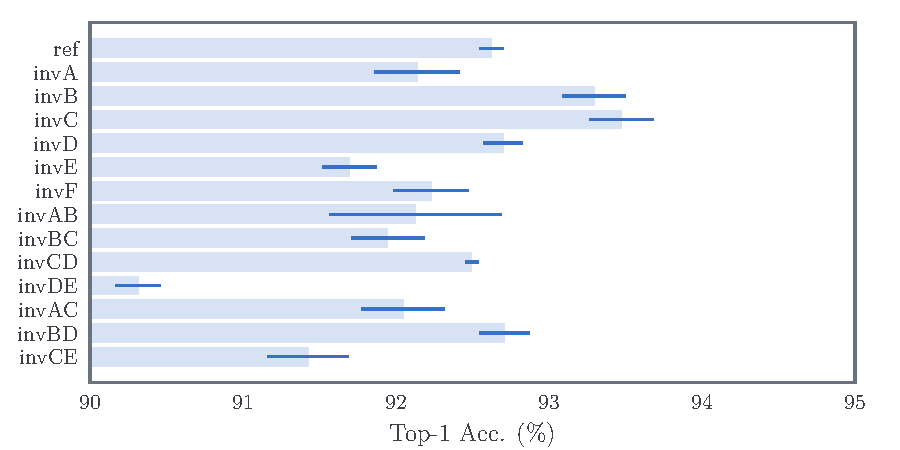
\includegraphics[width=\textwidth]{\imgpath/cifar10_invlayer.pdf}
    \label{fig:ch5:cifar10_invl}
  }\\
  \subfloat[CIFAR-100]{%
    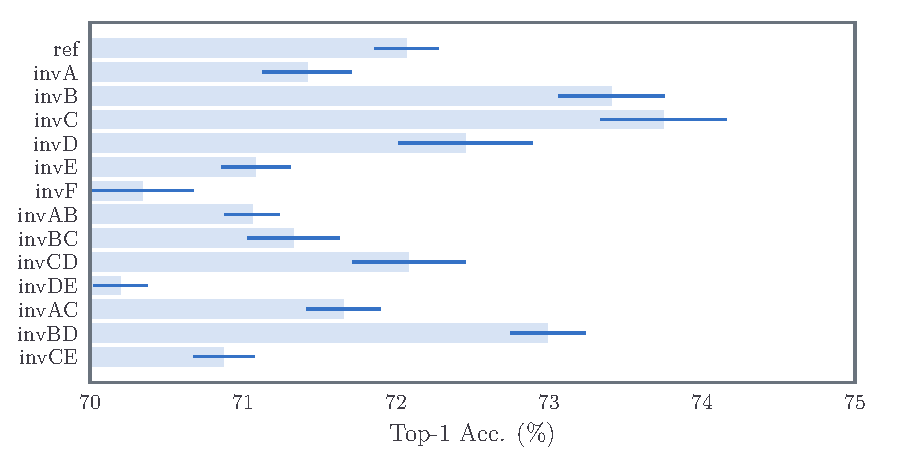
\includegraphics[width=\textwidth]{\imgpath/cifar100_invlayer.pdf}
    \label{fig:ch5:cifar100_invl}
  }
  % \subfloat[Tiny ImageNet]{%
    % 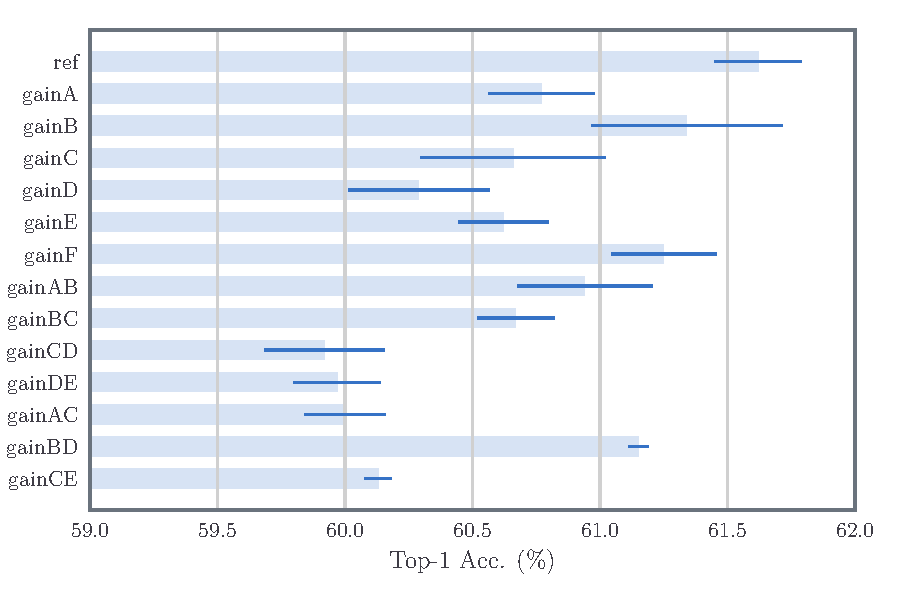
\includegraphics[width=0.8\textwidth]{\imgpath/ti_gainlayer.pdf}
    % \label{fig:ch6:ti_gl}
  % }\\
  \mycaption{Ablation results for the invariant layer}{Results for testing VGG like
  architecture with convolutional and invariant layers on several datasets.
  These graphs show the average top-1 accuracy on the validation set, and $\pm
  1$ standard deviation results (dark blue lines) for 5 runs. An architecture with `invX' means
  the equivalent convolutional layer `convX' from
  \autoref{tab:ch5:cifar_tiny_arch} was swapped for our proposed layer. The top
  row is the reference architecture using all convolutional layers. It appears
  that using a single invariant layer is the best option, and this will improve
  performance at many possible locations. The best position for the invariant
  layer appears to be around `convC', which is just after the first pooling
  layer.}
  \label{fig:ch5:inv_results}
\end{figure}

\begin{figure}[h!]
  \centering
  \subfloat[Tiny ImageNet]{%
    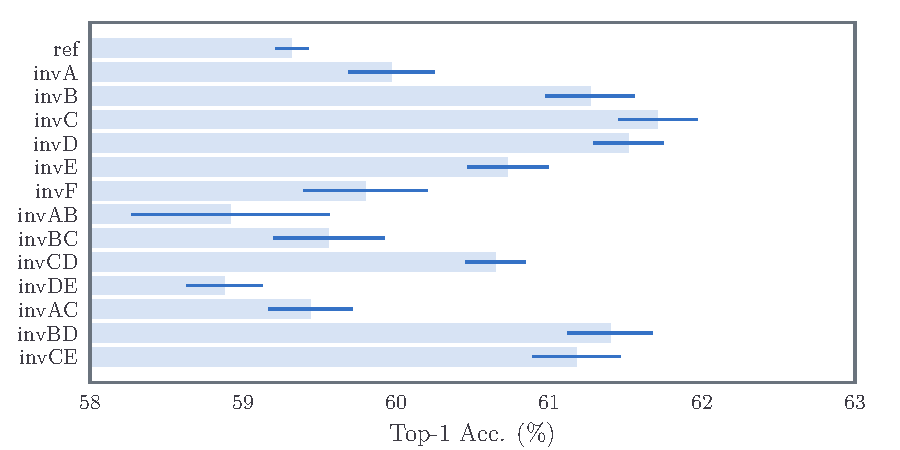
\includegraphics[width=\textwidth]{\imgpath/ti_invlayer.pdf}
    \label{fig:ch5:ti_invl}
    }
  % \subfloat[Tiny ImageNet]{%
    % 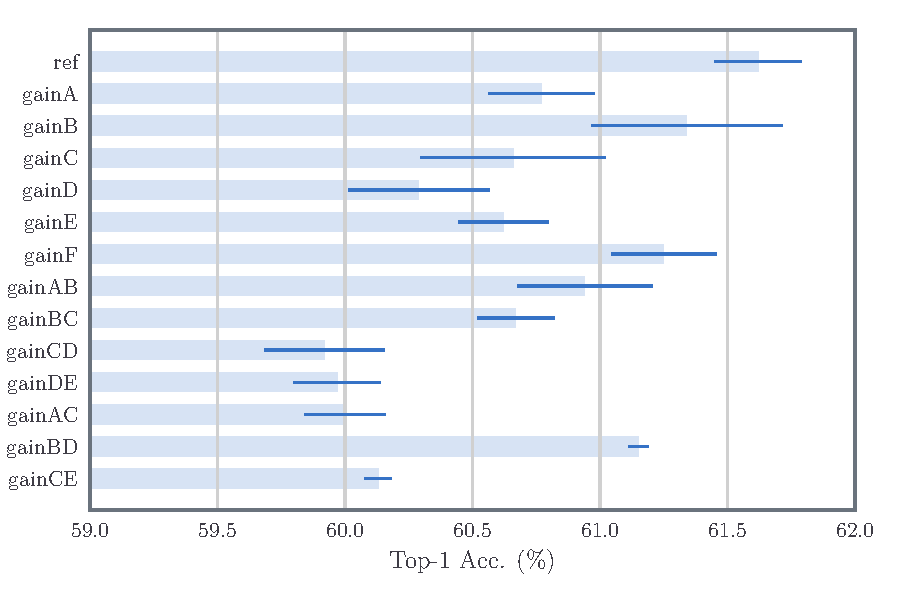
\includegraphics[width=0.8\textwidth]{\imgpath/ti_gainlayer.pdf}
    % \label{fig:ch6:ti_gl}
  % }\\
    \mycaption{Ablation results for Tiny ImageNet}{These graphs show the average
    top-1 accuracy on the validation set, and $\pm 1$ standard deviation results
    (dark blue lines) for 3 runs. Like with CIFAR, it appears gains can be made
    by using the invariant layer at least once in the network.  The best place
    for it appears to be around the first drop in resolution (which happens
    between `convB' and `convC').}
  \label{fig:ch5:inv_results_ti}
\end{figure}

We see improvements for all three datasets for many possible locations for the
invariant layer. The best permutations happen when one or two invariant layers are used
near the start of a system, but \emph{not} for the first layer. In particular, the best
position for the invariant layer seems to be when we remove the first max
pooling layer and use the natural downsampling of the invariant layer (at either
the `convB' or `convC' position). This also worked for the second pooling layer
(at the `convD' position), but having an invariant layer at both of these
positions (i.e. `convBD' and `convCE') performed slightly worse than using only one.

We recall that the magnitude operation in the ScatterNet effectively
demodulates the energy from higher spatial frequencies to lower ones. This
perhaps may explain why the best place for learnable scattering layers
are at positions where you want to downsample in a network.

We also tested the variations from \autoref{sec:ch5:mnist_newlayer} that added
spatial offsets to the gain layer by a fixed kernel and saw similar, if not
slightly worse, results than those in \autoref{fig:ch5:inv_results} and
\autoref{fig:ch5:inv_results_ti}. We did not
have time to explore fully as to why this was the case, but we believe that the
convolutional backend in the reference architecture (\autoref{tab:ch5:cifar_tiny_arch})
provided the necessary spatial separation to build rich shapes, something that
we did not have in the MNIST experiments.

\section{A New Hybrid ScatterNet}\label{sec:ch5:scat_exp}
\begin{table}[t]
  \renewcommand{\arraystretch}{1.2}
  \centering
  \mycaption{Hybrid ScatterNet models}{
  Hybrid ScatterNet architectures used for experiments on CIFAR-10 and
  CIFAR-100. For the reference architecture we show the front and back ends. The
  ScatNet A and ScatNet B architectures use the same back end as the reference.
  $N_c$ is the number of output classes; in our experiments we set the channel
  multiplier to be $C=96$.}
  \label{tab:ch5:cifar_arch2}
  \subfloat[Reference 1]{%
    \label{tab:ch5:net_ref}
    \begin{tabular}{l l}
      \toprule
      Layer & Act. Size \\\midrule
      \begin{tabular}{@{}l@{}}
        convA, $w\in \reals[21\x 3 \x 3\x 3]$ \\
        pool1, max pool $2\x 2$ \\
        convB, $w\in \reals[147\x 21\x 3\x 3]$\\ 
        pool2, max pool $2\x 2$ \\
      \end{tabular} &
      \begin{tabular}{@{}l@{}}
        $3\x 32\x 32$ \\ $21 \x 32\x 32$ \\ $21 \x 16\x 16$ \\ $147\x 16\x 16$ \\
        $147\x 8 \x 8$ \\ 
      \end{tabular}\\ \midrule 
      \begin{tabular}{@{}l@{}}
        convC, $w\in \reals[2C\x 147\x 3\x 3]$ \\
        convD, $w\in \reals[2C\x 2C\x 3\x 3]$ \\
        convE, $w\in \reals[4C\x 2C\x 3\x 3]$ \\
        convF, $w\in \reals[4C\x 4C\x 3\x 3]$ \\
        avg pool $8\x 8$ \\
        fc1, $4C\x N_c$
      \end{tabular} & 
      \begin{tabular}{@{}l@{}}
        \\$2C\x 8\x 8$ \\$2C\x 8\x 8$ \\$4C\x 8\x 8$ \\$4C\x 8\x 8$ \\
        $4C$ \\ $N_c$ \\
      \end{tabular}\\
      \bottomrule
    \end{tabular}
    } \\
  \subfloat[ScatNet A Front End]{%
    \label{tab:ch5:net_scatA}
    \begin{tabular}{l l}
      \toprule
      Layer & Act. Size \\\midrule
      \begin{tabular}{@{}l@{}}
        scat1, no $w$ \\
        scat2, no $w$ \\
      \end{tabular} &
      \begin{tabular}{@{}l@{}}
        $3\x 32\x 32$ \\ $21 \x 16\x 16$ \\ $147\x 8 \x 8$ \\
      \end{tabular}\\
      \bottomrule
    \end{tabular}
  }
  \subfloat[ScatNet B Front End]{%
    \label{tab:ch5:net_scatB}
    \begin{tabular}{l l}
      \toprule
      Layer & Act. Size \\\midrule
      \begin{tabular}{@{}l@{}}
        inv1, $A \in \reals[21\x 21]$ \\
        inv2, $A \in \reals[147\x 147]$ \\
      \end{tabular} &
      \begin{tabular}{@{}l@{}}
        $3\x 32\x 32$ \\ $21 \x 16\x 16$ \\ $147\x 8 \x 8$ \\
      \end{tabular}\\
      \bottomrule
    \end{tabular}
  } 
\end{table}
\begin{table}[t]
  \renewcommand{\arraystretch}{1.2}
  \centering
  \mycaption{Hybrid ScatterNet models with convolutional layer
  first}{New front ends for 3 models. The two ScatNet models are the same
  learnable scatternet from \autoref{tab:ch5:net_scatB} but with a small
  convolutional layer (`conv0') before it. ScatNet C ensures the same $147\x 8\x
  8$ output size as the models in \autoref{tab:ch5:cifar_arch2} but ScatNet D
  has a larger output size, allowing for the natural growth of a second-order
  ScatterNet model from $C$ input channels to $49C$ output channels.}
  \subfloat[Reference 2]{%
    \label{tab:ch5:net_ref2}
    \begin{tabular}{l l}
      \toprule
      Layer & Act. Size \\\midrule
      \begin{tabular}{@{}l@{}}
        conv0, $w\in \reals[16\x 3\x 3\x 3]$ \\
        convA, $w\in \reals[50\x 16\x 3\x 3]$ \\
        pool1, max pooling $2\x 2$ \\
        convB, $w\in \reals[147\x 50\x 3\x 3]$\\ 
        pool2, max pooling $2\x 2$ \\
      \end{tabular} &
      \begin{tabular}{@{}l@{}}
        $3\x 32\x 32$ \\ $16\x 32\x 32$ \\ $50 \x 32\x 32$ \\ $50 \x 16\x 16$ \\ $147\x 16\x 16$ \\
        $147\x 8 \x 8$ \\
      \end{tabular}\\
      \bottomrule
    \end{tabular}
  }\\
  \subfloat[ScatNet C]{%
    \label{tab:ch5:net_scatC}
    \begin{tabular}{l l}
      \toprule
      Layer & Act. Size \\\midrule
      \begin{tabular}{@{}l@{}}
        conv0, $w\in \reals[16\x 3\x 3\x 3]$ \\
        inv1, $A \in \reals[50\x 112]$ \\
        inv2, $A \in \reals[147\x 350]$ \\
      \end{tabular} &
      \begin{tabular}{@{}l@{}}
        $3\x 32\x 32$ \\ $16\x 32\x 32$ \\ $50 \x 16\x 16$ \\ $147\x 8 \x 8$ \\
      \end{tabular}\\
      \bottomrule
    \end{tabular}
  }  
  \subfloat[ScatNet D]{%
    \label{tab:ch5:net_scatD}
    \begin{tabular}{l l}
      \toprule
      Layer & Act. Size \\\midrule
      \begin{tabular}{@{}l@{}}
        conv0, $w\in \reals[16\x 3\x 3\x 3]$ \\
        inv1, $A \in \reals[112\x 112]$ \\
        inv2, $A \in \reals[784\x 784]$ \\
      \end{tabular} &
      \begin{tabular}{@{}l@{}}
        $3\x 32\x 32$ \\ $16\x 32\x 32$ \\ $112 \x 16\x 16$ \\ $784\x 8 \x 8$ \\
      \end{tabular}\\
      \bottomrule
    \end{tabular}
  }  
\end{table}


In the previous section, we examined how the locally invariant layer performs when
directly swapped for a convolutional layer in a CNN-based architecture.
In this section, we look at how it performs in a hybrid ScatterNet-like network
\cite{oyallon_scaling_2017}. Recall that a ScatterNet
naturally increases the channel dimension while downsampling the spatial
dimensions. A single scattering order for our $\DTCWT$ ScatterNet increases the channel dimension 
seven-fold and reduces the spatial area by four. After two layers of a
ScatterNet, the output has $49$ times more channels than the input and
one-sixteenth the spatial size.

We allow for this natural channel growth, using a ScatterNet front-end before
four convolutional layers similar to `convC' to `convF' from
\autoref{tab:ch5:cifar_tiny_arch}. The input to `convC' already has spatial size
$8\x 8$ so we do not need the pooling layer between `convD' and `convE'. The
final classification layer is the same global $8\x 8$ max pooling followed by a
fully connected layer. In addition, we use dropout in these later convolutional
layers with drop probability $p=0.3$. See \autoref{tab:ch5:net_ref} for the
backend layout. 

We compare a ScatterNet with no learning in between scattering orders (ScatNet A
in \autoref{tab:ch5:net_scatA}) to one with our proposal for a learned mixing
matrix (ScatNet B in \autoref{tab:ch5:net_scatB}). 
% For completeness, we
% compare these architectures for a similarly shaped convolutional frontend
% (Reference 1 in \autoref{tab:ch5:net_ref}).

We also test the hypothesis from \autoref{sec:ch5:conv_exp} that scattering layers may 
work better after the first layer of a network. To do this, we put a small
learned convolutional layer before the learnable ScatterNet front-end that takes the
three colour inputs and outputs 16 new channels. Increasing the ScatterNet input
to 16 channels means the default output size would be $16\x 49=784$ channels.
This is quite large, so we also use a system that uses a non-square $A$ matrix
for the two learnable invariant layers, keeping the output to 147 channels. We call this
option ScatNet C (see \autoref{tab:ch5:net_scatC}), and the full option with 
$784$ output channels ScatNet D (see \autoref{tab:ch5:net_scatD}). 

See
\autoref{tab:ch5:hybrid_scat} for the performance on CIFAR and
\autoref{tab:ch5:hybrid_scat_ti} for the performance on Tiny ImageNet.
For comparison, we have also listed the performance of other architectures on
CIFAR as reported by their authors in order of increasing complexity in
\autoref{tab:ch5:hybrid_scat}. 

The learnable invariant layer significantly improves the hybrid ScatterNets on
all three datasets (see the improvements from ScatNet A to ScatNet B).
As we anticipated, adding a learned layer before the learnable ScatterNet
improves things further, with ScatNet C and ScatNet D both having improvements on
ScatNets A and B.

Our proposed ScatNet C and ScatNet D achieve
comparable performance with the the All Conv, VGG16 and FitNet architectures.
The Deep\cite{he_deep_2016} and Wide\cite{zagoruyko_wide_2016} ResNets perform
best, but with very many more multiplies, parameters and layers.

ScatNets C and D perform marginally worse than the `invC' architecture from
\autoref{sec:ch5:conv_exp} but recall that the network is
quite different in these experiments - its front end is wider and has smaller
spatial support. The earlier reduction in spatial size in ScatNet C and D
meant that these networks took much less time to train
than those in the previous section (roughly 30 minutes for ScatNets A and B
compared to 2 to 4 hours for the networks in \autoref{sec:ch5:conv_exp} using
the hardware described in \autoref{app:arch}).

% ScatNet A underperforms the 
% fully convolutional reference architecture with the same shape, suggesting that
% using a fixed ScatterNet as a front-end may be no better than simply learning the front-end.
% However, the proposed learnable ScatterNet outperforms both ScatNet A and the reference
% architecture on all datasets, suggesting that it is important to mix across the
% Scattering channels.

% For comparison, we have also listed the performance of other architectures as
% reported by their authors in order of increasing complexity. 
% A final note we would like to make is that the proposed hybrid ScatterNet networks 
% architectures (particularly ScatNets C and ScatNets D) achieve near
% state-of-the-art performance even though they reduce the spatial size by a
% factor of 16 after only two layers. 
%and
%being quick to train --- dropping the spatial size to $8\x 8$ on CIFAR after
%only two layers is unique to the ScatterNet design. 

% ScatNets A to D with 6 layers like convC to convG from \autoref{tab:ch5:cifar_tiny_arch} after
% the scattering, achieve $58.1, 59.6, 60.8$ and $62.1\%$ top-1 accuracy on Tiny ImageNet. As
% these have more parameters and multiplies from the extra layers we exclude them
% from \autoref{tab:hybrid_scat}.

\begin{table}
  \renewcommand{\arraystretch}{1.2}
  \centering
  \mycaption{Hybrid ScatterNet top-1 classification accuracies on CIFAR}{ 
  $N_l$ is the number of learned convolutional layers, \#param is the number of
  parameters, and \#mults is the number of multiplies per $3\x 32\x 32$ image. An asterisk indicates
  that the value was estimated from the architecture description.}\label{tab:ch5:hybrid_scat}
  % \hspace{-10pt}
  \begin{tabular}{@{}lccccccc@{}}
  % \begin{tabular}{@{}llllllll@{}}
    \toprule
    & \multicolumn{3}{c}{Arch. Properties} && \multicolumn{3}{c}{Top 1 Accuracies (\%)} \\\cline{2-4}\cline{6-7}
    Arch. Name \phantom{abcde} & $N_l$ &\#Mparam &\#Mmults&\phantom{ab}&CIFAR-10&CIFAR-100\\ \midrule
    Reference 1 & 6 & 2.65 & 165 && 91.2 & 70.0 \\ 
    ScatNet A & 4 & 2.60 & 165 && 89.5 & 68.2 \\ 
    ScatNet B & 6 & 2.64 & 167 && 91.5 & 70.5  \\\midrule %
    Reference 2 & 7 & 2.69 & 165 && 92.2 & 72.2  \\ 
    ScatNet C & 7 & 2.64 & 251 && 92.6 & 72.7  \\ 
    ScatNet D & 7 & 3.7 & 251 && 93.3 & 73.6 \\ \midrule 
    All Conv\cite{springenberg_striving_2014-3} & 8 & 1.4 & 281\textsuperscript{*} && 92.8 & 66.3 \\ %    & - \\
    VGG16\cite{liu_very_2015} & 16 & 138\textsuperscript{*} & 313\textsuperscript{*}  && 91.6 & -  \\ 
    FitNet\cite{romero_fitnets:_2014} & 19 & 2.5 & 382 && 91.6 & 65.0 \\ %  & - \\
    % ResNet-110\cite{he_deep_2016} & 109 & 1.7 & 255\textsuperscript{*}& 93.6 & 74.8 \\ %              &  -\\
    ResNet-1001\cite{he_identity_2016} & 1000 & 10.2 & 4453\textsuperscript{*}&& 95.1 & 77.3 \\ %              &  -\\
    WRN-28-10\cite{zagoruyko_wide_2016} & 28 & 36.5 & 5900\textsuperscript{*} && 96.1 & 81.2 \\ %    & - \\
    \bottomrule
  \end{tabular}
  \\\vspace{20pt}
  \mycaption{Hybrid ScatterNet top-1 classification accuracies on Tiny ImageNet}{ 
  $N_l$ is the number of learned convolutional layers, \#param is the number of
  parameters, and \#mults is the number of multiplies per $32\x 32\x 3$ image. An asterisk indicates
  that the value was estimated from the architecture description.}\label{tab:ch5:hybrid_scat_ti}
  \begin{tabular}{@{}llc@{}}
    \toprule
    Arch. Name & \phantom{abc} & Top-1 Acc (\%)\\\midrule
    Reference1 && \\
    ScatNet A && \\
    ScatNet B && \\\midrule
    Reference 2 && \\
    ScatNet C && \\
    ScatNet D && \\ \bottomrule
  \end{tabular}
\end{table}


